

\section{Effort planning and review, TODO}

Effort planning and review are carried out to plan and confirm the time allocated to each phase. Additionally, this provides confirmation of the effort structure. Furthermore, it establishes the framework for a later review of the planned hours.



\subsection*{Effort planning}

The effort was planned according to the duration of the phases. These were laid out in the previous section and provide a start and end time for each phase. Thus, each phase contains a defined number of weeks. The planned effort is therefore first measured as an absolute number of weeks. Using this count, a relative effort is obtained by comparing the number of weeks per phase with the total number of weeks planned. Which results in the following formula to get the relative time allocation per phase. 

\[
\text{Relative time allocation}_i =
\frac{\text{Weeks allocated to phase } i}
{\text{Total planned weeks}} \times 100\%
\]



In the upcoming table, the relevant data for the calculation of the phase efforts is detailed. Phases always end according to the two-week sprint rhythm but do not necessarily end with the phase's last milestone. The table shows the following information:

\begin{itemize}
    \item \textbf{Phase:} The number of the phase for each line
    \item \textbf{Milestone:} This is either the milestone number or "end" in case it is the end of a phase.
    \item \textbf{MS date:} The date of the milestone or phase end date
    \item \textbf{Name of milestone:} The abbreviated name of the milestone or the end of a phase
    \item \textbf{Phase weeks total:} The total number of weeks spent in that phase
    \item \textbf{Relative percent:} According to the above formula, what percentage of the total time is spent in this phase.
\end{itemize}

\begin{table}[htbp]
    \centering
    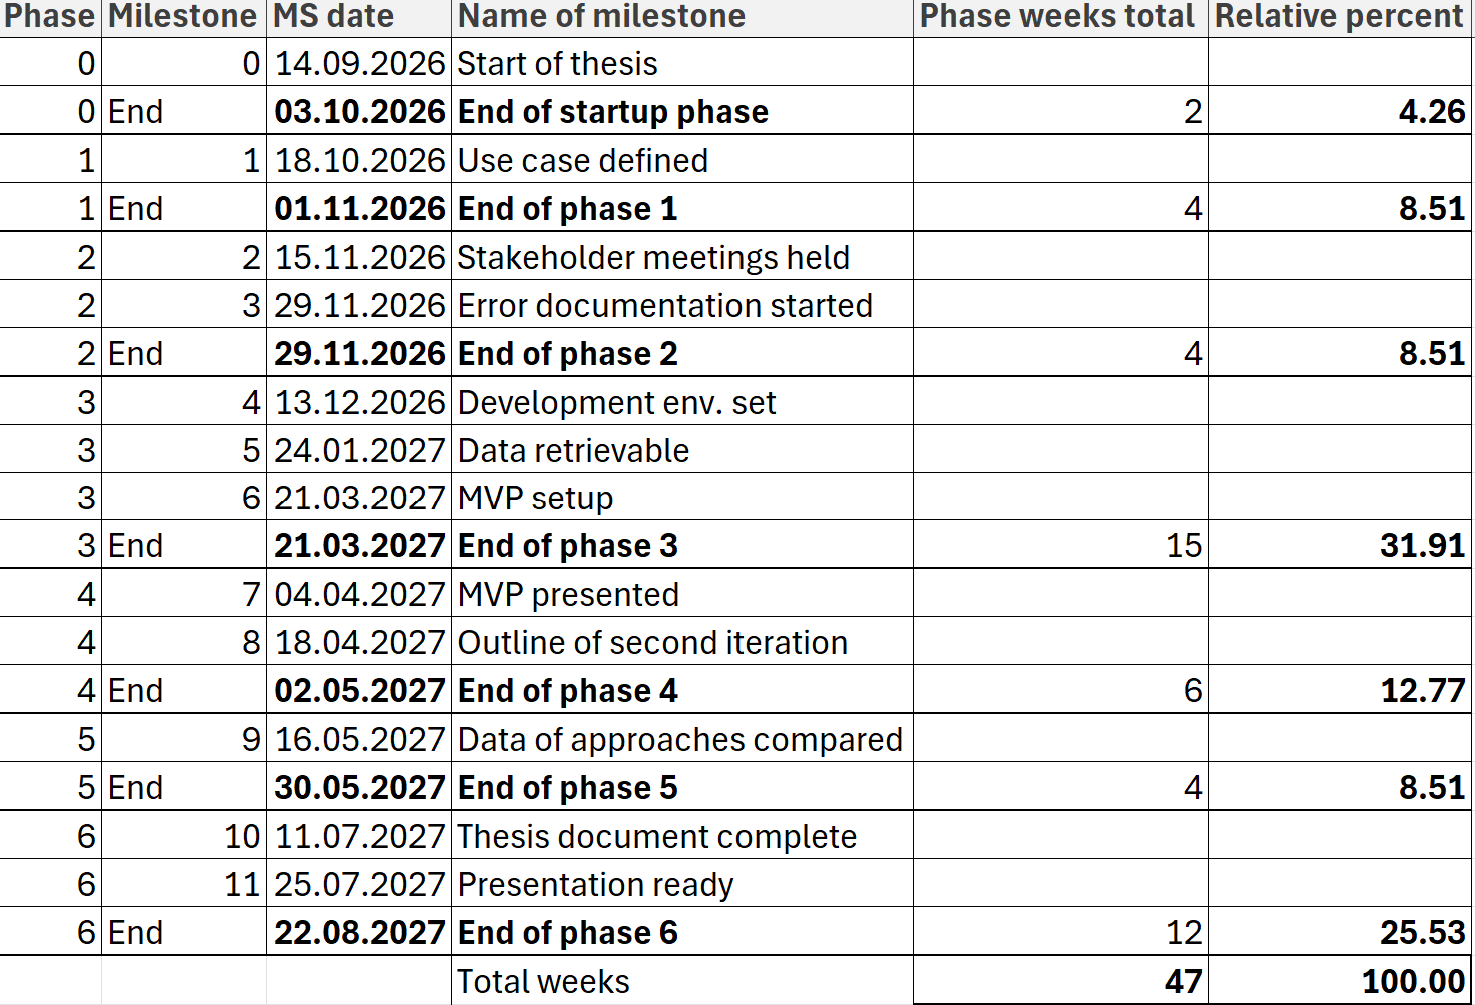
\includegraphics[width=\textwidth]{./content/img/Mth/ProjectManagement/TimeLinePercentage.png}
    \caption{Distribution of planned project duration across project phases}
    \label{tab:timeline_percentage}
\end{table}




\subsection*{Two ways of recorded time}
First to some rules as to how time can be registered. Regarding work efforts its important to note that the academic team has an agreement with Swiss Post defining which efforts are considered work time and which not. 
As per agreement, the research part and the writing part of this document are not to be noted as work time, however the remainder of activities such as implementation, documenting work state in Jira or confluence etc. are considered work efforts and are noted into the time tracking at swiss post as such. 

This agreement leads to two different ways of tracking time. At Swiss Post, time is tracked directly with their SAP time-tracking \gls{MIAR} system, where the efforts are recorded against a specific project account. This makes it easy to export and track them for monitoring purposes in the thesis.

Second, academic efforts committed to the project outside the agreement were recorded separately. The work was then registered in blocks of continuous work on project-related tasks, including short breaks. However, longer breaks, such as lunch, resulted in a new block being created.


\subsection*{Planning review}
At the end of the thesis, the number of hours tracked is summed up per phase, based on the start and end dates that were actually reached, taking into account any deviations. These totals per phase and the overall total lead to a second relative measure. The two relative measures per phase are then compared and evaluated. A summary of this is provided along with the analysis of the planning process at the end of this project management chapter.
